\documentclass{beamer}

\usepackage{amsmath}
\usepackage{amssymb}
\usepackage{xcolor}

\usetheme{Madrid}
\title[Crisis]{Mastering the game of Go with deep neural networks and tree search}
\subtitle{Understanding Monte Carlo Tree Search (MCTS)}
\author{Naren Sundaravaradan}
\institute{Unifie}
\date{Papers We Love, Bengaluru, 2019}

\begin{document}
\frame{\titlepage}

\section{Introduction}

\begin{frame}
  \frametitle{What's the paper about?}
  \begin{itemize}
  \item Introduces an algorithm that plays the game of Go at the highest level.
    \pause
  \item The algorithm introduced is easily generalizable to other games.
    \pause
  \item It makes use of the existing Monte Carlo Tree Search (MCTS) algorithm and enhances it using heuristics learnt through deep learning.
  \end{itemize}
\end{frame}

\begin{frame}
  \frametitle{What we will cover}
  \begin{itemize}
  \item Describe a simpler two-player game to help illustrate the paper better
    \pause
  \item Derive and explore the optimal gameplay algorithm (minimax).
    \pause
  \item Derive and explore vanilla MCTS
    \pause
  \item Understand the Exploration-Exploitation tradeoff using Upper Confidence Trees (UCT)
    \pause
  \item Describe MCTS as used in the paper
  \end{itemize}
\end{frame}

\section{Optimal Gameplay}

\begin{frame}
  \frametitle{Greedy-Coins Game}
  \begin{columns}[c]
    \column{.5\textwidth}
    \begin{itemize}
    \item Found in the 2012 Midsouth Programming Contest \url{http://ccsc-ms.org/2012_Problems/index.html}
      \pause
    \item The aim is to collect coins worth more than that collected by the opponent
      \pause
    \item Only one coin is picked on each turn from either the left or the right
    \end{itemize}
    \column{.5\textwidth}
    \begin{figure}[h]
      \centering
      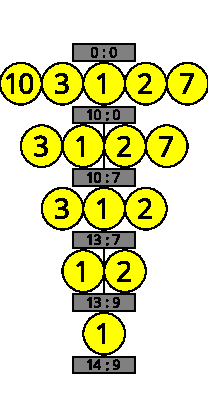
\includegraphics{figs/examples/one.pdf}
    \end{figure}
  \end{columns}
\end{frame}

\begin{frame}
  \frametitle{The Game Tree}
  \begin{figure}[h]
    \centering
    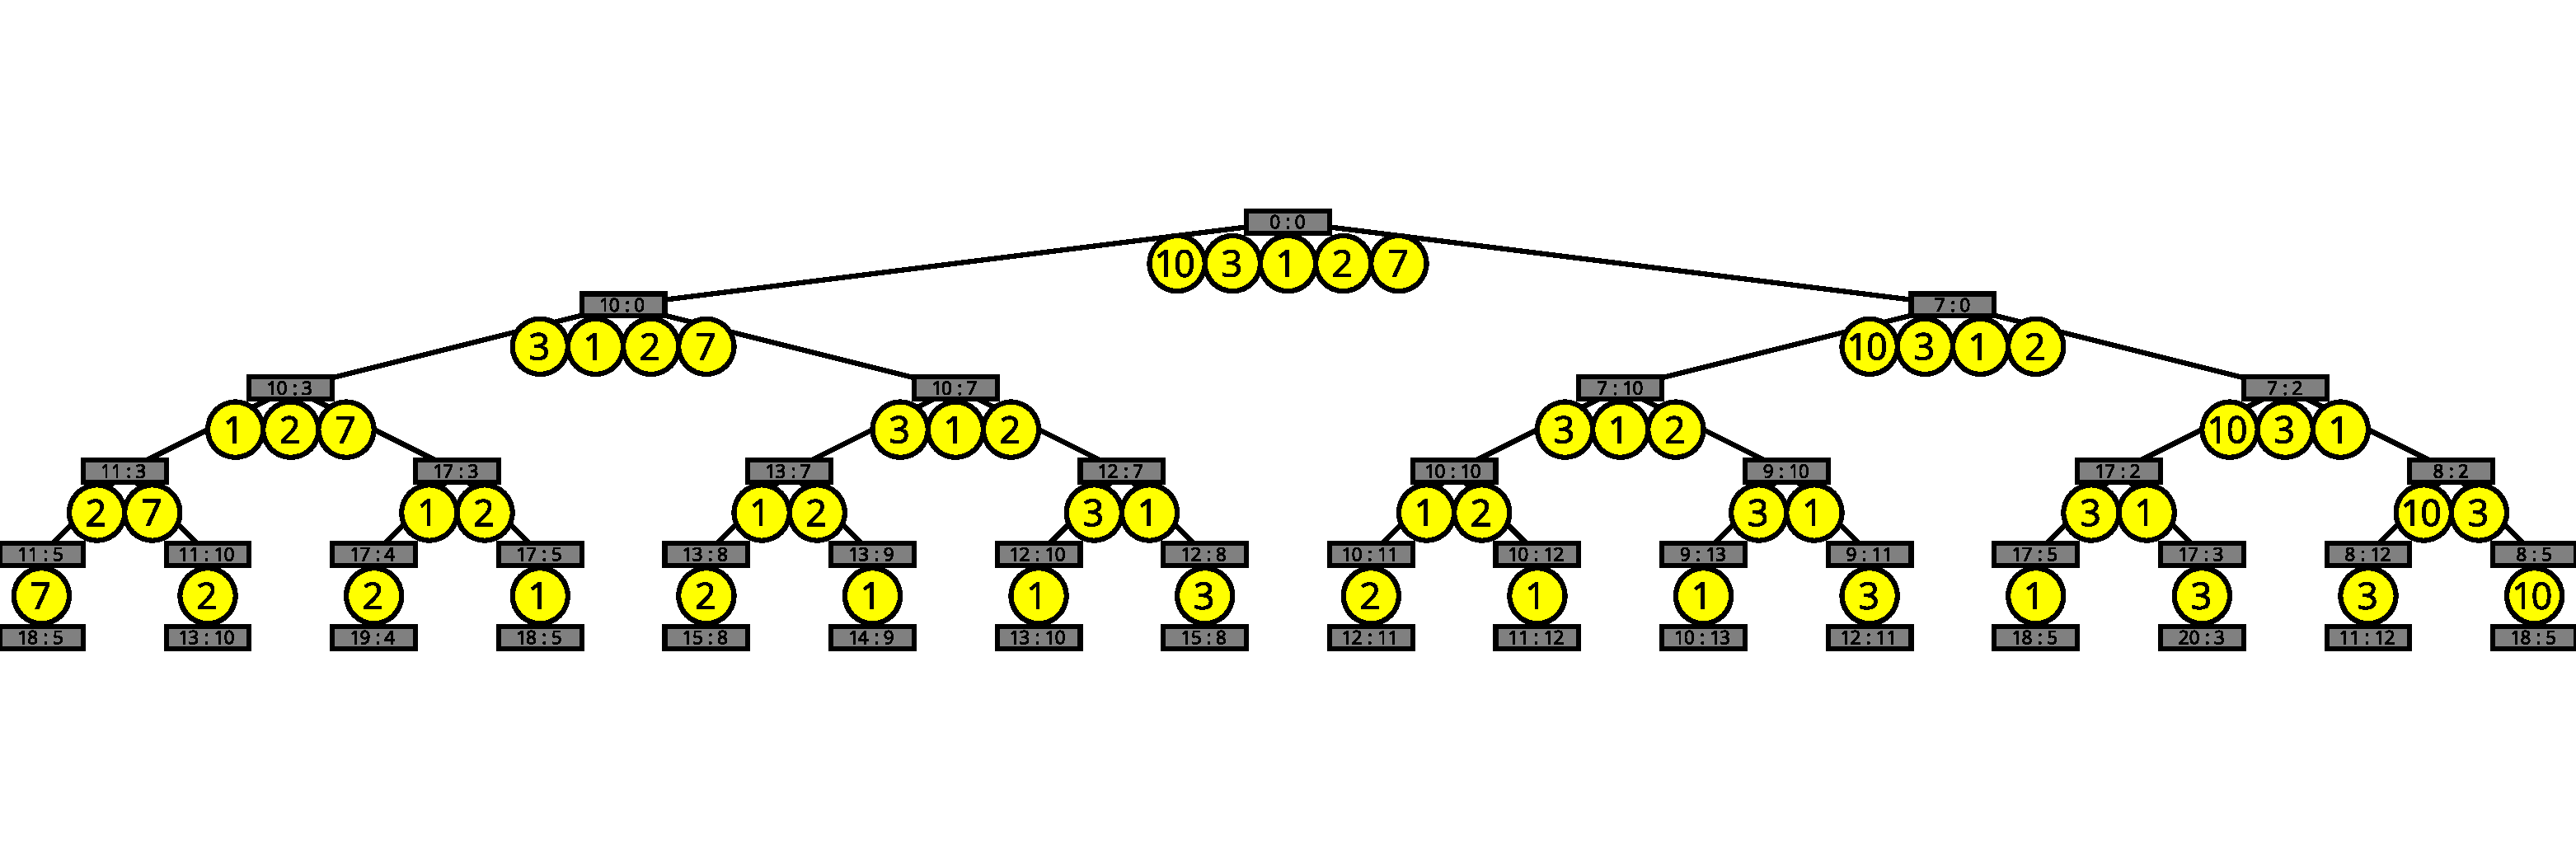
\includegraphics[width=0.95\textwidth]{figs/examples/full.pdf}
  \end{figure}
\end{frame}

\begin{frame}
  \frametitle{Minimax}
  \begin{itemize}
  \item Is an algorithm to play \emph{optimally}. It picks the move that achieves the best score \emph{assuming} the opponent also plays \emph{optimally}.
  \pause
  \item Mathematically, if $s$ is the current state, then the best move $a \in A(s)$ is the one that maximizes
  \end{itemize}
  \pause
  \begin{displaymath}
    \text{best score} | s = \underset{a_1 \in A}{\begingroup\color{red}\max\endgroup} \left(\text{ best acheivable score } | a_1, s\right)
  \end{displaymath}
  \pause
  \begin{itemize}
  \item But what is the right-hand side?
  \end{itemize}
  \pause
  \begin{displaymath}
    \text{best score} | a_1, s = \underset{a_2 \in A}{\begingroup\color{red}\min\endgroup} \left(\text{ best acheivable score } | a_2, a_1, s\right)
  \end{displaymath}
  \pause
  \begin{itemize}
  \item Keep recursing until the right-hand side has no more moves to make
  \end{itemize}
  \pause
  \begin{displaymath}
    \text{best score} | a_n,\dots,a_1, s = \text{final score for player} | a_n, \dots, a_1, s
  \end{displaymath}
\end{frame}

\begin{frame}
  \frametitle{Minimax Demo}
  \begin{center}
    See \textbf{examples/minimax}
  \end{center}
\end{frame}

\begin{frame}
  \frametitle{Limitations of minimax}
  \begin{itemize}
  \item Game trees are large!
    \pause
  \item Chess has a branching factor of around $35$ and depth of around $80$, that's $35^{80}$ games to explore.
    \pause
  \item Go has a branching factor of around $250$ and depth of around $150$.
    \pause
  \item Even our game becomes infeasible if w start with a large number of coins.
    \pause
  \item \textbf{However}, minimax requires no knowledge beyond the rules of the game!
  \end{itemize}
\end{frame}

\begin{frame}
  \frametitle{What if we run minimax on a subset of games?}
  \begin{center}
      Good moves are much rarer than bad ones and are easy to miss when sampled randomly.
  \end{center}
\end{frame}

\section{Monte Carlo Tree Search}

\begin{frame}
  \frametitle{Monte Carlo Tree Search: What do we want?}
  \begin{itemize}
  \item We want to know the probability of winning on board $s$ given \emph{optimal} play.
  \end{itemize}
  \pause
  \begin{displaymath}
    P(\text{win} | s) = \sum_{a_1, \dots, a_N} \text{isWin}(a_1,\dots, a_N | s)P^*(a_1, \dots, a_N | s)
  \end{displaymath}
  \pause
  \begin{itemize}
  \item But what is $P^*(a | s) $? It is the probability that the move $a$ is optimal. We do not know this!
  \pause
  \item We, however, do know that
  \end{itemize}
  \begin{displaymath}
    P^*(a | s) = \frac{P(\text{win} | a, s)}{\sum_{a\in A(s)} P(\text{win} | a, s)}
  \end{displaymath}
  \pause
  \begin{itemize}    
  \item We have now defined the RHS in terms of a smaller LHS. We can solve for $P^*(a | s)$.
  \end{itemize}
\end{frame}

\begin{frame}
  \frametitle{Monte Carlo Tree Search}
  \begin{itemize}
  \item Below is a possible method for solving for $P^*(a | s)$.
    \pause
  \item Starting at board $s$, play a few games, $\{G_a^1, G_a^2, \dots, G_a^k\}$ for each possible first move $a \in A(s)$ followed by random moves till the end.
  \pause
  \item We can use the result of these games to give us an estimate for the probability of winning if we start with move $a$, $P_e(\text{win} | a, s)$ since
  \end{itemize}
  \pause
  \begin{displaymath}
    P_e(\text{win} | a, s) = \frac{1}{k}\sum_{i=1}^k \text{isWin}(G_a^i)
  \end{displaymath}
  \begin{itemize}
  \item Now that we have $P(\text{win} | a, s)$ for $a \in A(s)$, we can estimate $P(a | s)$ using the formula for $P^*(a | s)$.
    \pause
  \item Now, the next time we play a few more games don't choose the first move randomly but choose it according to $P_e(\text{win} | a, s)$.
    \pause
  \item Monte Carlo tells us that this process (repeated) guarantees that $P(a | s) \longrightarrow P^*(a | s)$.
  \end{itemize}
\end{frame}

\begin{frame}
  \frametitle{Monte Carlo Tree Search: Example}
  \begin{center}
    See \textbf{examples/vanilla}
  \end{center}
\end{frame}

\begin{frame}
  \frametitle{Monte Carlo Tree Search: Limitations}
  \begin{center}
    It can take a long time for $P(a | s) \longrightarrow P^*(a | s)$
  \end{center}
\end{frame}

\section{Speeding Up MCTS}

\begin{frame}
  \frametitle{Speeding up MCTS: Upper Confidence Trees}
  \begin{itemize}
  \item Consider ten slot machine each having a jackpot probability given by $P^*(\text{win} | M_i)$ which we don't know.
    \pause
  \item What is the best strategy for you to figure out $P^*(\text{win} | M_i)$ while \emph{minimizing} your losses?
    \pause
  \item The MCTS we described is not the best strategy.
    \pause
  \item A strategy called Upper Confidence Trees picks the next machine to play by seeing which machine has the highest following value
  \end{itemize}
  \pause
  \begin{align*}
    &\frac{1}{N_i}\sum_{j=1}^{N_i} x_{ij} + \sqrt{\frac{2\ln \sum_i N_i}{N_i}}\\
    &N_i = \text{number of times machine } i \text{ is played}\\
    &x_{ij} = \text{win or loss when playing machine } i \text{ the jth time}
  \end{align*}
\end{frame}

\begin{frame}
  \frametitle{Speeding up MCTS: Example}
  \begin{center}
    See \textbf{examples/uct}
  \end{center}
\end{frame}

\begin{frame}
  \frametitle{Speeding up MCTS: AlphaGo}
  \begin{itemize}
  \item Even MCTS with UCT has a few limitations.
    \pause
  \item First, when we got to a leaf node, we end up playing random games again.
    \pause
  \item The solution is to use a heuristic that can give \emph{quick}
    indications of which moves should be preferred. AlphaGo achieves
    this using a deep learning model trained against human-expert
    moves from $30$ million games.
    \pause
  \item Second, when a move is selected, UCT uses no prior knowledge of gameplay to make a better decision.
    \pause
  \item AlphaGo uses a prior distribution of moves learnt by a deep
    learning model using reinforcement learning and human-expert moves.
  \end{itemize}
\end{frame}

\begin{frame}
  \frametitle{Speeding up MCTS: AlphaGo Example}
  \begin{center}
    See \textbf{examples/alphago}
  \end{center}
\end{frame}

\begin{frame}
  \frametitle{Thank You}
  \begin{center}
    \url{https://github.com/nanonaren/PWL_AlphaGo}
  \end{center}
\end{frame}

\end{document}
